% SC4002 Chapter 6: Sequence-to-Sequence --- Encoder-Decoder, Attention, Beam Search (0->100)
\chapter[Seq2Seq: Encoder-Decoder and Attention]{Sequence-to-Sequence Learning: Encoder-Decoder, Attention, and Beam Search}
\label{ch:seq2seq}

\begin{quote}
\emph{``To translate you must first understand, then generate---but how much can you squeeze through a single vector?''} --- This chapter compresses a sentence into a bottleneck, then learns to look back.
\end{quote}

\noindent\fbox{\parbox{\dimexpr\linewidth-2\fboxsep-2\fboxrule}{%
\textbf{From zero: no seq2seq background assumed.} We start from translation as mapping one sequence to another of different length, build the encoder-decoder RNN, diagnose its bottleneck, fix it with attention (Bahdanau and Luong), and decode with beam search. Every formula is motivated by a picture first.}}
\vspace{0.4em}

\section*{Learning Outcomes}
After this chapter you will be able to:
\begin{enumerate}[label=(L\arabic*)]
    \item formulate machine translation as seq2seq and explain the fixed-vector bottleneck;
    \item write encoder and decoder recurrences and the factorization $P(\mathbf{y}\mid\mathbf{x})$;
    \item derive attention weights $\alpha_{ij}=\mathrm{softmax}(\mathrm{score})$ and the context vector $\mathbf{c}_i$ in Bahdanau and Luong variants;
    \item run beam search with width $k$ and contrast it with greedy decoding;
    \item describe BLEU and teacher forcing and why they matter forSeq2Seq training.
\end{enumerate}

% ============================================================
\section{Translation as Seq2Seq: The Bottleneck Problem}
\label{sec:bottleneck}
\paragraph{Intuition.} Translation maps ``\emph{le chat dort}'' $\to$ ``\emph{the cat sleeps}''---input and output have different lengths, no word-to-word alignment is given, and order may change. Seq2seq treats it as: read the whole French sentence, remember its meaning, then write English one word at a time. The earliest solution compressed everything into one vector $\mathbf{c}$: the encoder's last hidden state.

\paragraph{Why this hurts.} Imagine summarizing a 30-word sentence into a single 512-dimensional vector and then reproducing it perfectly. Information is lost---the bottleneck. Long sentences degrade first; the decoder's first steps see the same $\mathbf{c}$ as its last steps, with no way to re-inspect the source. Performance on WMT translation visibly drops past 20 tokens without a fix.

\paragraph{Example.} Source $\mathbf{x}=(x_1,x_2,x_3)=(\text{le},\text{chat},\text{dort})$, target $\mathbf{y}=(y_1,y_2,y_3)=(\text{the},\text{cat},\text{sleeps})$. We need a model for $P(\mathbf{y}\mid\mathbf{x})=\prod_{t=1}^{T_y} P(y_t\mid y_{<t},\mathbf{x})$ that works for any $T_y\neq T_x$.

% ============================================================
\section{The Encoder-Decoder Architecture}
\label{sec:encdec}
\paragraph{Formal definition.} Let source embeddings $\mathbf{e}^x_t$ and target embeddings $\mathbf{e}^y_t$. The \emph{encoder} is an RNN (vanilla, GRU, or LSTM):
\begin{equation}
\mathbf{h}_t = f_{\text{enc}}(\mathbf{e}^x_t, \mathbf{h}_{t-1}),\quad t=1,\dots,T_x,\quad \mathbf{c}=\mathbf{h}_{T_x},
\label{eq:encoder}
\end{equation}
with variants: bidirectional $\mathbf{h}_t=[\overrightarrow{\mathbf{h}}_t;\overleftarrow{\mathbf{h}}_t]$. The \emph{decoder} generates autoregressively:
\begin{equation}
\mathbf{s}_t = f_{\text{dec}}(\mathbf{e}^y_{t-1}, \mathbf{s}_{t-1}, \mathbf{c}),\quad P(y_t\mid y_{<t},\mathbf{x})=\mathrm{softmax}(W_o\mathbf{s}_t+\mathbf{b}_o)_{y_t},
\label{eq:decoder}
\end{equation}
with $\mathbf{s}_0=\mathbf{c}$ and $y_0=\langle\text{s}\rangle$. Training maximizes $\sum_{(\mathbf{x},\mathbf{y})}\log P(\mathbf{y}\mid\mathbf{x})$ via teacher forcing (feed gold $y_{t-1}$). Fig.~\ref{fig:encdec-bottleneck} shows the bottleneck.

\begin{figure}[h]
\centering
\begin{tikzpicture}[
  enc/.style={rectangle, draw=blue!65!black, thick, fill=blue!15, minimum width=1.2cm, minimum height=0.7cm, font=\scriptsize, rounded corners=2pt},
  dec/.style={rectangle, draw=green!55!black, thick, fill=green!15, minimum width=1.2cm, minimum height=0.7cm, font=\scriptsize, rounded corners=2pt},
  vec/.style={rectangle, draw=red!65!black, thick, fill=red!12, minimum width=0.7cm, minimum height=1.1cm, font=\tiny, rounded corners=3pt, align=center},
  lab/.style={font=\tiny, color=gray!70!black},
  arr/.style={-{Latex[length=2.2mm]}, thick, color=gray!70!black},
  arrb/.style={-{Latex[length=2.2mm]}, thick, color=red!60!black}
]
% source words
\node[lab] at (0,1.8) {Source: \emph{le chat dort}};
\node[enc] (e1) at (0,0.9) {$\mathbf{h}_1$}; \node[enc] (e2) at (1.7,0.9) {$\mathbf{h}_2$}; \node[enc] (e3) at (3.4,0.9) {$\mathbf{h}_3$};
\node[lab] at (0,0.35) {$x_1$}; \node[lab] at (1.7,0.35) {$x_2$}; \node[lab] at (3.4,0.35) {$x_3$};
\draw[arr, blue!60!black] (e1)--(e2); \draw[arr, blue!60!black] (e2)--(e3);
% bottleneck
\node[vec] (c) at (5.2,0.9) {$\mathbf{c}$\\$\mathbf{h}_{T_x}$};
\draw[arrb] (e3)--(c) node[midway, above, font=\tiny, fill=red!8, rounded corners=1pt] {squeeze};
% decoder
\node[dec] (d1) at (7.0,0.9) {$\mathbf{s}_1$}; \node[dec] (d2) at (8.7,0.9) {$\mathbf{s}_2$}; \node[dec] (d3) at (10.4,0.9) {$\mathbf{s}_3$};
\draw[arr, green!55!black] (c)--(d1); \draw[arr, green!55!black] (d1)--(d2); \draw[arr, green!55!black] (d2)--(d3);
\node[lab] at (7.0,0.35) {$y_1$=the}; \node[lab] at (8.7,0.35) {$y_2$=cat}; \node[lab] at (10.4,0.35) {$y_3$=sleeps};
% dashed context reuse
\draw[arr, dashed, red!50!black, opacity=0.6] (c.south) -- ++(0,-0.55) -| (d2.south);
\draw[arr, dashed, red!50!black, opacity=0.6] (c.south) -- ++(0,-0.75) -| (d3.south);
\node[font=\tiny, fill=yellow!10, draw=gray!40, rounded corners=2pt, inner sep=2pt] at (5.2,-0.7) {fixed $\mathbf{c}$ reused every step};
\node[font=\tiny, fill=blue!8, draw=gray!30, rounded corners=2pt, inner sep=2pt] at (1.7,2.25) {\textcolor{blue!60!black}{$\blacksquare$ encoder} \; \textcolor{red!60!black}{$\blacksquare$ bottleneck} \; \textcolor{green!55!black}{$\blacksquare$ decoder}};
\end{tikzpicture}
\caption{Encoder-decoder bottleneck. The encoder compresses $\mathbf{x}$ into a single vector $\mathbf{c}=\mathbf{h}_{T_x}$ (red); the decoder sees only $\mathbf{c}$ at every step. Long inputs lose detail---attention will let the decoder re-read all $\mathbf{h}_j$.}
\label{fig:encdec-bottleneck}
\end{figure}

Without attention the model must memorize word order, agreement, and alignment inside $\mathbf{c}$ alone, which fails for $T_x\gg 10$.

% ============================================================
\section{Attention: Letting the Decoder Look Back}
\label{sec:attention}
\paragraph{Intuition.} A human translator does not memorize the French sentence and then close the book. She glances back at relevant source words while writing each English word. Attention gives the decoder the same ability: at step $i$ it computes a weighted average of \emph{all} encoder states, focusing on the useful positions.

\paragraph{Formal mechanism.} Keep all encoder states $\mathbf{h}_1,\dots,\mathbf{h}_{T_x}$. At decoder step $i$ with state $\mathbf{s}_{i-1}$:
\begin{align}
e_{ij} &= \mathrm{score}(\mathbf{s}_{i-1}, \mathbf{h}_j) &&\text{alignment score} \label{eq:score}\\
\alpha_{ij} &= \frac{\exp(e_{ij})}{\sum_{k=1}^{T_x}\exp(e_{ik})} = \mathrm{softmax}_j(e_{ij}) &&\text{attention weight, } \sum_j\alpha_{ij}=1 \label{eq:alpha}\\
\mathbf{c}_i &= \sum_{j=1}^{T_x} \alpha_{ij}\,\mathbf{h}_j &&\text{context vector (dynamic)} \label{eq:context}\\
\mathbf{s}_i &= f_{\text{dec}}(\mathbf{e}^y_{i-1}, \mathbf{s}_{i-1}, \mathbf{c}_i),\quad P(y_i\mid y_{<i},\mathbf{x})=\mathrm{softmax}(W_o[\mathbf{s}_i;\mathbf{c}_i]) . \label{eq:att-dec}
\end{align}
Two scoring variants:
\begin{equation}
\text{Bahdanau: } e_{ij}=\mathbf{v}_a^\top\tanh(W_a\mathbf{s}_{i-1}+U_a\mathbf{h}_j),\quad
\text{Luong: } e_{ij}=\mathbf{s}_{i-1}^\top W_a\mathbf{h}_j\ (\text{general}) \text{ or } \mathbf{s}_{i-1}^\top\mathbf{h}_j\ (\text{dot}).
\label{eq:score-variants}
\end{equation}
Bahdanau (additive) feeds $[\mathbf{s}_i;\mathbf{c}_i]$ into the output; Luong (multiplicative) often uses $\tilde{\mathbf{s}}_i=\tanh(W_c[\mathbf{s}_i;\mathbf{c}_i])$. Fig.~\ref{fig:att-heatmap} visualizes $\alpha_{ij}$.

\begin{figure}[h]
\centering
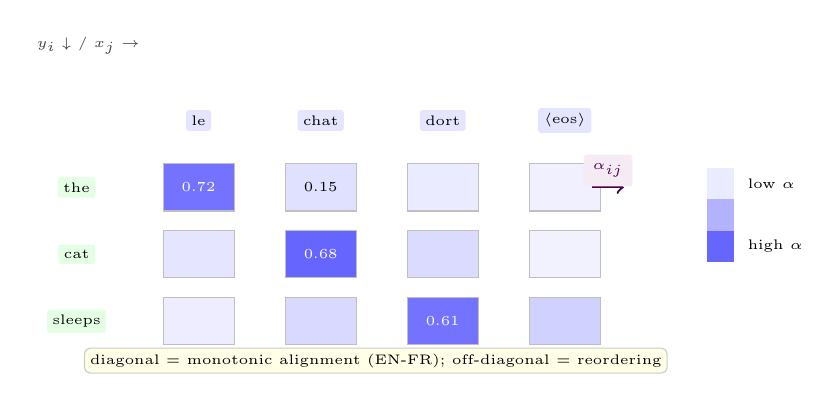
\begin{tikzpicture}[font=\scriptsize]
% grid: 4 source cols (le, chat, dort, <eos>) x 3 target rows (the, cat, sleeps)
\foreach \j/\lab in {1/le,2/chat,3/dort,4/{$\langle$eos$\rangle$}} {
  \node[font=\tiny, fill=blue!10, rounded corners=1pt, inner sep=2pt] at (\j*1.55,3.0) {\lab};
}
\foreach \i/\lab in {1/the,2/cat,3/sleeps} {
  \node[font=\tiny, fill=green!10, rounded corners=1pt, inner sep=2pt] at (0,3.0-\i*0.85) {\lab};
}
% attention weights (example plausible alignment)
% row1 the -> le (high), row2 cat->chat, row3 sleeps->dort
\fill[blue!55] (1*1.55-0.45,3.0-1*0.85-0.3) rectangle (1*1.55+0.45,3.0-1*0.85+0.3);
\fill[blue!12] (2*1.55-0.45,3.0-1*0.85-0.3) rectangle (2*1.55+0.45,3.0-1*0.85+0.3);
\fill[blue!8]  (3*1.55-0.45,3.0-1*0.85-0.3) rectangle (3*1.55+0.45,3.0-1*0.85+0.3);
\fill[blue!6]  (4*1.55-0.45,3.0-1*0.85-0.3) rectangle (4*1.55+0.45,3.0-1*0.85+0.3);

\fill[blue!10] (1*1.55-0.45,3.0-2*0.85-0.3) rectangle (1*1.55+0.45,3.0-2*0.85+0.3);
\fill[blue!60] (2*1.55-0.45,3.0-2*0.85-0.3) rectangle (2*1.55+0.45,3.0-2*0.85+0.3);
\fill[blue!14] (3*1.55-0.45,3.0-2*0.85-0.3) rectangle (3*1.55+0.45,3.0-2*0.85+0.3);
\fill[blue!5]  (4*1.55-0.45,3.0-2*0.85-0.3) rectangle (4*1.55+0.45,3.0-2*0.85+0.3);

\fill[blue!7]  (1*1.55-0.45,3.0-3*0.85-0.3) rectangle (1*1.55+0.45,3.0-3*0.85+0.3);
\fill[blue!15] (2*1.55-0.45,3.0-3*0.85-0.3) rectangle (2*1.55+0.45,3.0-3*0.85+0.3);
\fill[blue!55] (3*1.55-0.45,3.0-3*0.85-0.3) rectangle (3*1.55+0.45,3.0-3*0.85+0.3);
\fill[blue!18] (4*1.55-0.45,3.0-3*0.85-0.3) rectangle (4*1.55+0.45,3.0-3*0.85+0.3);
% grid lines
\foreach \i in {1,2,3} \foreach \j in {1,2,3,4} {
  \draw[gray!50, thin] (\j*1.55-0.45,3.0-\i*0.85-0.3) rectangle (\j*1.55+0.45,3.0-\i*0.85+0.3);
}
% alpha values
\node[font=\tiny, white] at (1*1.55,3.0-1*0.85) {0.72}; \node[font=\tiny] at (2*1.55,3.0-1*0.85) {0.15};
\node[font=\tiny, white] at (2*1.55,3.0-2*0.85) {0.68}; \node[font=\tiny, white] at (3*1.55,3.0-3*0.85) {0.61};
\node[font=\tiny, gray!50!black] at (0.15,3.95) {$y_i\downarrow$ / $x_j\to$};
% color bar
\fill[blue!8] (8.0,2.4) rectangle (8.35,2.0); \fill[blue!30] (8.0,2.0) rectangle (8.35,1.6); \fill[blue!60] (8.0,1.6) rectangle (8.35,1.2);
\node[font=\tiny, right] at (8.4,2.2) {low $\alpha$}; \node[font=\tiny, right] at (8.4,1.4) {high $\alpha$};
\node[font=\tiny, fill=yellow!10, draw=gray!40, rounded corners=2pt, inner sep=2pt] at (3.8,-0.05) {diagonal = monotonic alignment (EN-FR); off-diagonal = reordering};
\draw[->, thick, violet!60!black] (6.55,2.15) -- (6.95,2.15) node[midway, above, font=\tiny, fill=violet!8, rounded corners=1pt] {$\alpha_{ij}$};
\end{tikzpicture}
\caption{Attention heatmap $\alpha_{ij}$ for \emph{le chat dort} $\to$ \emph{the cat sleeps}. Each row sums to 1 (softmax). Bright diagonal shows the model attends to the corresponding source word; context $\mathbf{c}_i$ is the $\alpha$-weighted sum of all $\mathbf{h}_j$.}
\label{fig:att-heatmap}
\end{figure}

Attention removes the bottleneck: $\mathbf{c}_i$ is recomputed each step, gradients flow directly to the relevant $\mathbf{h}_j$, and alignment becomes interpretable.

% ============================================================
\section{Decoding with Beam Search and Training}
\label{sec:beam-bleu}
\paragraph{Greedy vs.\ beam search.} Greedy decoding picks $\hat{y}_t=\arg\max P(y_t\mid\hat{y}_{<t},\mathbf{x})$---locally optimal, globally myopic. Beam search keeps the top-$k$ hypotheses (beam width $k$), expanding each by $|V|$ words and pruning to $k$ best by log-probability:
\begin{equation}
\mathrm{score}(\mathbf{y}_{1:t})=\sum_{i=1}^{t}\log P(y_i\mid y_{<i},\mathbf{x}),\quad \mathcal{B}_t=\mathrm{top}_k\{\mathrm{score}(\mathbf{y})\mid \mathbf{y}\in \mathcal{B}_{t-1}\times V\}.
\label{eq:beam}
\end{equation}
With $k=1$ this is greedy; $k=5$--$10$ is typical. Hypotheses ending in $\langle\text{eos}\rangle$ are complete; we normalize by length $(1/T)^\alpha$ to avoid short-sequence bias. Fig.~\ref{fig:beam-tree} traces $k=2$.

\paragraph{Training and BLEU.} Training uses teacher forcing and cross-entropy on $P(\mathbf{y}\mid\mathbf{x})$. At test time we report BLEU: geometric mean of $n$-gram precisions ($n=1..4$) times brevity penalty $\mathrm{BP}=\exp(1-r/c)$ if $c<r$ (candidate shorter than reference). BLEU correlates with human judgment but penalizes paraphrases; it is not differentiable, so we train on likelihood and evaluate on BLEU.

\begin{figure}[h]
\centering
\begin{tikzpicture}[
  hyp/.style={rectangle, draw=blue!60!black, thick, fill=blue!12, rounded corners=3pt, minimum width=1.3cm, minimum height=0.6cm, font=\scriptsize},
  hyp2/.style={rectangle, draw=green!55!black, thick, fill=green!14, rounded corners=3pt, minimum width=1.3cm, minimum height=0.6cm, font=\scriptsize},
  hyp3/.style={rectangle, draw=orange!60!black, thick, fill=orange!14, rounded corners=3pt, minimum width=1.3cm, minimum height=0.6cm, font=\scriptsize},
  pruned/.style={rectangle, draw=gray!50, thick, fill=gray!10, rounded corners=3pt, minimum width=1.3cm, minimum height=0.6cm, font=\scriptsize, dashed},
  arr/.style={-{Latex[length=2mm]}, thick},
  scorelab/.style={font=\tiny, fill=yellow!10, rounded corners=1pt, inner sep=1.5pt}
]
\node[hyp] (root) at (0,3.8) {$\langle$s$\rangle$ 0.0};
% t=1 expansions (k=2 keep top 2)
\node[hyp] (a1) at (-2.2,2.6) {the $-0.2$}; \node[hyp2] (a2) at (2.2,2.6) {a $-0.8$}; \node[pruned] (a3) at (5.0,2.6) {le $-2.1$};
\draw[arr, blue!60!black] (root)--(a1); \draw[arr, green!55!black] (root)--(a2); \draw[arr, gray!50, dashed] (root)--(a3);
\node[scorelab] at (5.0,2.05) {pruned};
% t=2 from "the"
\node[hyp] (b1) at (-3.4,1.3) {cat $-0.5$}; \node[hyp2] (b2) at (-1.0,1.3) {dog $-1.4$}; 
% t=2 from "a"
\node[hyp3] (b3) at (1.6,1.3) {cat $-1.1$}; \node[pruned] (b4) at (4.2,1.3) {dog $-2.0$};
\draw[arr, blue!60!black] (a1)--(b1); \draw[arr, gray!50, dashed] (a1)--(b2);
\draw[arr, orange!60!black] (a2)--(b3); \draw[arr, gray!50, dashed] (a2)--(b4);
% candidates ranked at t=2: the cat (-0.5), a cat (-1.1) kept; others pruned
\node[font=\tiny, fill=blue!8, draw=gray!30, rounded corners=2pt, inner sep=2pt] at (-2.2,0.65) {beam $k{=}2$: keep top 2};
% t=3 continuations
\node[hyp] (c1) at (-3.4,0.0) {sleeps $-0.7$}; \node[hyp3] (c2) at (1.6,0.0) {sleeps $-1.5$};
\draw[arr, blue!60!black] (b1)--(c1); \draw[arr, orange!60!black] (b3)--(c2);
\node[font=\tiny, fill=green!8, draw=green!40, rounded corners=2pt, inner sep=2pt] at (6.8,0.5) {$\checkmark$ best: the cat sleeps};
% baseline greedy path annotation
\node[font=\tiny, fill=red!8, rounded corners=1pt, inner sep=2pt, align=left] at (-6.2,1.3) {greedy\\would pick\\the $\to$ cat\\(same here,\\not always)};
\end{tikzpicture}
\caption{Beam search with width $k=2$. Each level expands $k\times|V|$ candidates, keeps the $k$ highest $\sum\log P$. Pruned hypotheses (dashed gray) are discarded. Completed hypotheses are length-normalized before final selection; greedy ($k=1$) can miss the global optimum.}
\label{fig:beam-tree}
\end{figure}

\begin{lstlisting}[language=Python, caption={Attention weights and beam search (width $k$) for seq2seq. Bahdanau scores shown; swap in Luong dot-product easily.}, label={lst:att-beam}]
import numpy as np

def attention_scores(s_prev, H, Wa, Ua, va):
    """Bahdanau scores: s_prev (d), H (Tx,d) -> e (Tx,)"""
    # e_j = v_a^T tanh(W_a s + U_a h_j)
    proj_s = Wa @ s_prev          # (d,)
    proj_H = H @ Ua.T             # (Tx, d)
    e = np.tanh(proj_H + proj_s) @ va  # (Tx,)
    alpha = np.exp(e) / np.sum(np.exp(e))  # softmax Eq.12
    c = alpha @ H                  # (d,) context vector Eq.13
    return e, alpha, c

def beam_search(decode_step, enc_states, beam_width=2, max_len=10):
    """decode_step(beam_seq, context) -> dict{word: logprob}."""
    beams = [([0], 0.0)]  # (token_ids, logprob); 0 = <s>
    completed = []
    for t in range(max_len):
        candidates = []
        for seq, score in beams:
            if seq[-1] == 1:  # <eos> id=1, already complete
                completed.append((seq, score / len(seq)**0.6))  # length norm
                continue
            # recompute attention context for this hypothesis
            # (simplified: use last decoder state approximated by mean)
            logprobs = decode_step(seq, enc_states)  # {wid: logp}
            for wid, lp in logprobs.items():
                candidates.append((seq + [wid], score + lp))
        if not candidates:
            break
        candidates.sort(key=lambda x: x[1], reverse=True)
        beams = candidates[:beam_width]
        if len(completed) >= beam_width:
            break
    completed.extend((s, sc / len(s)**0.6) for s, sc in beams if s[-1]==1)
    best = max(completed or beams, key=lambda x: x[1])
    return best  # (best_seq, best_score)

# Tiny demo: Tx=3, d=4
np.random.seed(0)
H = np.random.randn(3, 4)
s = np.random.randn(4)
Wa, Ua = np.random.randn(4,4), np.random.randn(4,4)
va = np.random.randn(4)
e, alpha, c = attention_scores(s, H, Wa, Ua, va)
print(f"alpha={np.round(alpha,3)} sum={alpha.sum():.2f}")  # sums to 1
print(f"context shape {c.shape}")
\end{lstlisting}

% ============================================================
\section{Chapter Notes}
Sutskever, Vinyals and Le (2014) and Cho et al.\ (2014) introduced encoder-decoder RNNs for machine translation. Bahdanau, Cho and Bengio (2015) added additive attention to break the bottleneck, followed by Luong, Pham and Manning (2015) with multiplicative variants. Beam search analysis and length normalization tricks are standard in neural MT; BLEU was defined by Papineni et al.\ (2002). Attention paved the way for the Transformer.

% ============================================================
\section{Exercises}
\label{sec:ch06-exercises}
\begin{enumerate}[label=E6.\arabic*, leftmargin=*, itemsep=0.7em]
    \item \textbf{Bottleneck intuition.} Give a 25-word English sentence that a fixed-vector encoder-decoder is likely to mistranslate and explain which information the bottleneck would discard. How does attention avoid this loss?
    \item \textbf{Attention by hand.} Let $\mathbf{s}=[1,0]$, $\mathbf{h}_1=[1,1]$, $\mathbf{h}_2=[-1,1]$, Luong dot score $e_j=\mathbf{s}^\top\mathbf{h}_j$. Compute $e_1,e_2$, then $\alpha_1,\alpha_2=\mathrm{softmax}(e)$, then $\mathbf{c}=\sum_j\alpha_j\mathbf{h}_j$. Repeat with Bahdanau where $W_a=U_a=I$, $\mathbf{v}_a=[1,1]$.
    \item \textbf{Bahdanau vs.\ Luong.} State one advantage of Bahdanau additive scoring (hint: dimensions) and one of Luong dot-product (hint: speed). When $\mathbf{s}$ and $\mathbf{h}_j$ have different dimensions, which variants apply without projection?
    \item \textbf{Beam search trace.} Vocabulary $\{a,b,\langle\text{eos}\rangle\}$, $k=2$. At $t{=}1$: $P(a)=0.5, P(b)=0.3, P(\text{eos})=0.2$. From $a$: $P(a)=0.1,P(b)=0.1,P(\text{eos})=0.8$; from $b$: $P(a)=0.6,P(b)=0.2,P(\text{eos})=0.2$. Run beam search for two steps, list kept beams with scores, and compare the best beam to greedy.
    \item \textbf{BLEU and teacher forcing.} Compute BLEU-2 for candidate ``the cat cat'' vs.\ reference ``the cat sleeps'' with brevity penalty. Then explain \emph{exposure bias} from teacher forcing and one mitigation (scheduled sampling or minimum-risk/BLEU training).
\end{enumerate}
% End of Chapter 6
